%\documentclass[PhD]{iitmdiss}
%\documentclass[MS]{iitmdiss}
\documentclass[MTech]{iitmdiss}
%\documentclass[BTech]{iitmdiss}
\usepackage{times}
 \usepackage{t1enc}
 \usepackage{listings}

\usepackage{graphicx}
\graphicspath{ {ffigures/} }
\usepackage[hidelinks]{hyperref} % hyperlinks for references.
\usepackage{amsmath} % easier math formulae, align, subequations \ldots

\begin{document}

%%%%%%%%%%%%%%%%%%%%%%%%%%%%%%%%%%%%%%%%%%%%%%%%%%%%%%%%%%%%%%%%%%%%%%
% Title page

\title{CONTROL OF XYZ POSITIONING SYSTEM FOR MICRO-CT USING HC-05/RASPBERRY-PI
}

\author{CHIRANJEEVI SAITEJA DOMMETI}

\date{MONTH 2009}
\department{PHYSICS}

%\nocite{*}
\maketitle

%%%%%%%%%%%%%%%%%%%%%%%%%%%%%%%%%%%%%%%%%%%%%%%%%%%%%%%%%%%%%%%%%%%%%%
% Certificate
\certificate

\vspace*{0.5in}

\noindent This is to certify that the thesis titled {\bf \LaTeX\ CLASS  
  FOR DISSERTATIONS SUBMITTED TO IIT-M}, submitted by {\bf Author}, 
  to the Indian Institute of Technology, Madras, for
the award of the degree of {\bf Doctor of Philosophy}, is a bona fide
record of the research work done by him under our supervision.  The
contents of this thesis, in full or in parts, have not been submitted
to any other Institute or University for the award of any degree or
diploma.

\vspace*{1.5in}

\begin{singlespacing}
\hspace*{-0.25in}
\parbox{2.5in}{
\noindent {\bf Prof.~1} \\
\noindent Research Guide \\ 
\noindent Professor \\
\noindent Dept. of Physics\\
\noindent IIT-Madras, 600 036 \\
} 
\hspace*{1.0in} 
%\parbox{2.5in}{
%\noindent {\bf Prof.~S.~C.~Rajan} \\
%\noindent Research Guide \\ 
%\noindent Assistant Professor \\
%\noindent Dept.  of  Aerospace Engineering\\
%\noindent IIT-Madras, 600 036 \\
%}  
\end{singlespacing}
\vspace*{0.25in}
\noindent Place: Chennai\\
Date: 19th January 2009 


%%%%%%%%%%%%%%%%%%%%%%%%%%%%%%%%%%%%%%%%%%%%%%%%%%%%%%%%%%%%%%%%%%%%%%
% Acknowledgements
\acknowledgements

Firstly, I would like to thank my guide, Prof. Ganapathy Krishnamurthi Sir for giving me an opportunity to work on this project and for giving me any needed help and mentoring
along the way. Working on this project was a good learning experience, both
academically and personally.


I would like to thank my parents for the constant support they provided, especially at times I was feeling low.
A special thanks to my sister who somehow always knows the right course of action at any situation.

I would like to thank Swathi for all the support and time she has spent explaining stuff about the modules I have been working on throughout the project.

I would like to thank Srinivas and Sandeep for being there when I needed it
the most. A special thanks to Vamshi Pavan, Samba, Vamshi Gujjala, Vamsi Gatla, Abhishek Ananthula, Devanand, Venky, Rajeevi, Abhigyan, Akshay, Tilak and Koutilya ,Ajith and all my friends I made in the institute for making my stint a memorable one. I thank Rakesh, Pabu, for their immense support. All of your help was invaluable and I appreciate it heartfully.



%%%%%%%%%%%%%%%%%%%%%%%%%%%%%%%%%%%%%%%%%%%%%%%%%%%%%%%%%%%%%%%%%%%%%%
% Abstract

\abstract

\noindent KEYWORDS: \hspace*{0.5em} \parbox[t]{4.4in}{ Positioning System; Micro-CT; IoT;Arduino Controlled.}

\vspace*{24pt}

\noindent The development of automation industry, complex and multidisciplinary nature of research has led to the growth of remote interactive experimentation, monitoring and control. At the same time, the advancement in information technology has faced the challenges by increase in computation capabilities and internet bandwidths. 
Web-Based Control (WBC) involves controlling the remote devices via internet. It has captured a huge interest of real-world applications like monitoring and/or control in tele-manufacturing, tele-surgery, tele-robotics and distant education. Its architecture essentially comprise of remote devices, sensors, actuators, controllers, computers and communication networks. 

Every system is automated in order to face new challenges in present situation. Automated systems have less manual operations, so that the flexibility, reliabilities are high and accurate. Hence every field prefers automated control systems. Especially in the field of bio-medical electronics automated systems are doing better performance. Nowadays, there are lots of good-quality motor speed controls on the market. However, their costs are relatively high. A speed control with both low cost and good performance will be highly marketable, especially for small mobility applications. On the other hand, the wireless connectivity has a nature of low cost and less environmental limitations. The present trend IoT technology is better suitable for automation systems. 

A complete Arduino based system was made which would receive commands from a smartphone through bluetooth module (HC-05) and subsequently drive the stepper motors. These stepper motors drive the X,Y,Z axes


\pagebreak

%%%%%%%%%%%%%%%%%%%%%%%%%%%%%%%%%%%%%%%%%%%%%%%%%%%%%%%%%%%%%%%%%
% Table of contents etc.

\begin{singlespace}
\tableofcontents
\thispagestyle{empty}

\listoftables
\addcontentsline{toc}{chapter}{LIST OF TABLES}
\listoffigures
\addcontentsline{toc}{chapter}{LIST OF FIGURES}
\end{singlespace}


%%%%%%%%%%%%%%%%%%%%%%%%%%%%%%%%%%%%%%%%%%%%%%%%%%%%%%%%%%%%%%%%%%%%%%
% Abbreviations
\abbreviations

\noindent 
\begin{tabbing}
xxxxxxxxxxx \= xxxxxxxxxxxxxxxxxxxxxxxxxxxxxxxxxxxxxxxxxxxxxxxx \kill
\textbf{IITM}   \> Indian Institute of Technology, Madras \\
\textbf{RTFM} \> Read the Fine Manual \\
\end{tabbing}

\pagebreak

%%%%%%%%%%%%%%%%%%%%%%%%%%%%%%%%%%%%%%%%%%%%%%%%%%%%%%%%%%%%%%%%%%%%%%
% Notation

\chapter*{\centerline{NOTATION}}
\addcontentsline{toc}{chapter}{NOTATION}

\begin{singlespace}
\begin{tabbing}
xxxxxxxxxxx \= xxxxxxxxxxxxxxxxxxxxxxxxxxxxxxxxxxxxxxxxxxxxxxxx \kill
\textbf{$r$}  \> Radius, $m$ \\
\textbf{$\alpha$}  \> Angle of thesis in degrees \\
\textbf{$\beta$}   \> Flight path in degrees \\
\end{tabbing}
\end{singlespace}

\pagebreak
\clearpage

% The main text will follow from this point so set the page numbering
% to arabic from here on.
\pagenumbering{arabic}


%%%%%%%%%%%%%%%%%%%%%%%%%%%%%%%%%%%%%%%%%%%%%%%%%%
% Introduction.

\chapter{INTRODUCTION}
\label{chap:intro}

Every system is automated in order to face new challenges in present situation. Automated systems have less manual operations, so that the flexibility, reliabilities are high and accurate. Hence every field prefers automated control systems. Especially in the field of bio-medical electronics automated systems are doing better performance. Nowadays, there are lots of good-quality motor speed controls on the market. However, their costs are relatively high. A speed control with both low cost and good performance will be highly marketable, especially for small mobility applications. On the other hand, the wireless connectivity has a nature of low cost and less environmental limitations. The present trend IoT technology is better suitable for automation systems. 

The IoT refers to the ability of everyday objects to connect to the Internet and to send and receive data. It includes, for example, home automation systems that turn on your front porch light when you leave work; Internet-connected cameras that allow you to post pictures online with a single click; and bracelets that share with your friends how far you have biked or run during the day. IoT described it as including “embedded intelligence” in individual items that can detect changes in their physical state and control them too. IoT have in common is that focus on how computers, sensors, and objects interact with one another and process data. Internet of Things (IoT) becomes utility with increased sophistication in sensing, actuation, communication, control and in creating knowledge from vast amounts of data. It is rapidly increasing technology, the network of physical objects or things are interconnected with electronics. IoT has given us a promising way to build powerful industrial applications by using wireless devices, Android, and sensors. The physical objects that are being connected will possess one or more sensors. Each sensor will monitor a specific condition such as location, vibration, motion and temperature. In IoT, these sensors will connect to each other and to systems that can understand or present information from the sensor’s data feeds. 

The IoT concept was simple but powerful. If all objects in daily life were equipped with identifiers and wireless connectivity, these objects could be communicating with each other and be managed by computers. Stepper motors are strong, slow and accurate. Their strength and relatively slow speed means they can usually be used without any gear-down mechanisms. Their extreme accuracy makes them ideal for robotic applications. They can be easily obtained from old computer compact disk drives or printers. A traditional motor has a series of coils which are automatically switched on and off by a set of brushes in contact with the commutator (where the sparks and ozone come from). Once power is applied, the motor runs itself at a speed proportional to the voltage and the load. For as stepper motor there is no commutator. Instead, there are five or six wires coming out of the motor. Stepper motors are DC motors that move in discrete steps. They have multiple coils that are organized in groups called "phases". By energizing each phase in sequence, the motor will rotate one step at a time. With a computer controlled stepping you can achieve very precise positioning and/or speed control. For this reason, stepper motors are the motor of choice for many precision motion control applications. The main usage of stepper motor is positioning of stepper motor rotor rotates with required precision. Stepper motor is suitable for primarily tasks where the precision is very important factor. Application areas are automobile industry, computer hard disks, printers, tool machines, actuators of industry robots and manipulators etc. For stepper motor control it is necessary control unit, which generates steps of motor. Stepper motor is a special type of synchronous motor. The difference between the synchronous and stepper motor is stepper motor can reach certain amount of defined positions. The step of motor is reached by suitable activity of control unit. The basic principle of the motion is electric current flowing through the coil generates magnetic field. This magnetic field pulls opposite pole of rotor magnet. By suitable generating of pulses to coils, the rotor starts to rotate.


\section{OBJECTIVES}

\begin{itemize}
\item Propose a reliable economic alternative Gantry and XYZ positioning system
\item Decrease the workload on DaQ card partially or completely by leveraging the power of SoC (Arduino/Raspberry-Pi)
\item IoT-ize the System for remote access and control

\end{itemize}



\section{METHODOLOGY}

\subsection{\emph{Design of the Gantry Mechanism}}


The first task is to design and build a Gantry Mechanism. A model of the actual mechanism is built. The mechanism has four degrees of freedom: three along the coordinate axis X, Y and Z direction, and one rotation in the X-Y plane. The mechanism carries a payload and maneuvers it in the working space. The mechanical parts comprise of timing belt-pulley drives, screw-nut arrangements and the transmission shafts. The electrical parts are stepper motors, sensors, motor drivers and microcontroller unit.

\subsection{\emph{Decrease the workload on DaQ card partially or completely by leveraging the power of SoC (Arduino/Raspberry-Pi)}}

The idea is to make use of the recently available SoCs such as Arduino and the various options of Analog inputs/outputs and GPIOs to shed off or completely eliminate the processing on the costlier available DaQ cards and also on the LabView Software and GUI. Please refer to Fig.~\ref{joystic}

\begin{figure}[h!]
	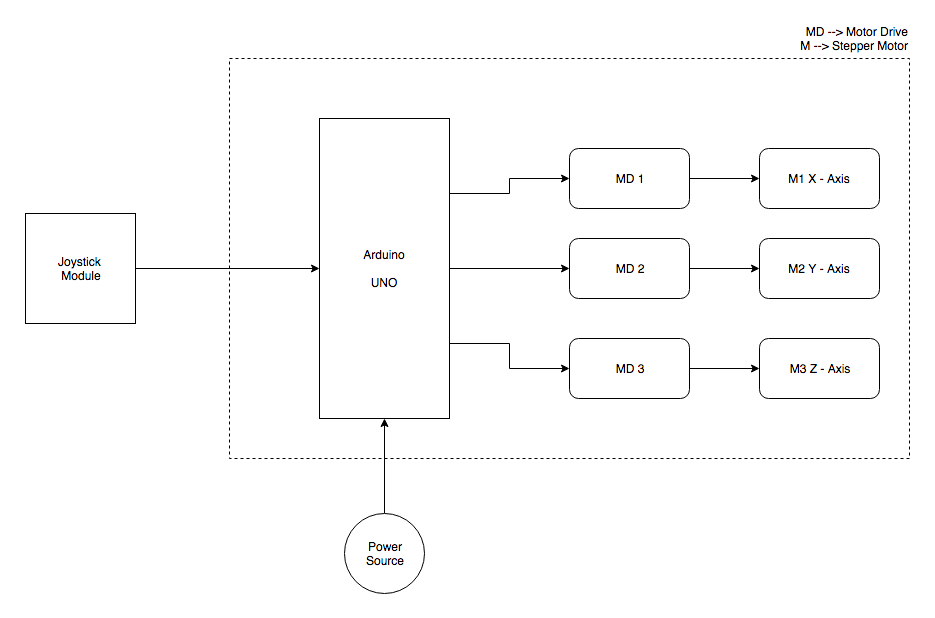
\includegraphics[width=\linewidth]{ffigures/joystick_diag}	
	\caption{ Joystick module connected to Arduino. The Arduino acts as the Controller to drive the stepper motors}
	\label{joystic}
\end{figure}

\subsection{\emph{IoT-ize the System for remote access and control
}}

IoT (Internet of Things) The Internet of Things (IoT) is the network of physical devices, vehicles, home appliances and other items embedded with electronics, software, sensors, actuators, and connectivity which enables these things to connect and exchange data, creating opportunities for more direct integration of the physical world into computer-based systems, resulting in efficiency improvements, economic benefits and reduced human intervention.

Raspberry Pi (RPi) is an SoC with a 64 bit quad core processor, and has onboard WiFi, Bluetooth and USB boot capabilities and other options including Power over Ethernet (PoE) and network boot (an SD card is no longer required). This allows the use of the Pi in hard-to-reach places (possibly without electricity)

\begin{figure}[h!]
	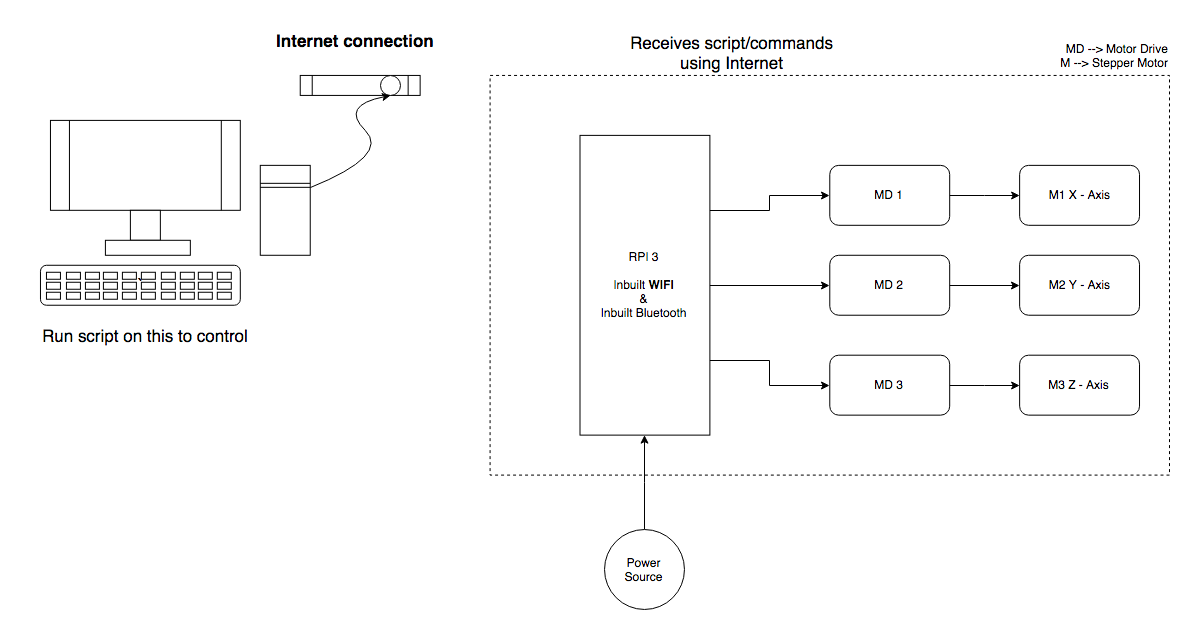
\includegraphics[width=\linewidth]{ffigures/rpi_diag}
	\caption{RPi Module connected to internet and receiving commands from a remote-PC}
	\label{rpi1}
\end{figure}

We install the Linux image on the RPi and boot it into Linux operating system. The RPi and Linux environments help us in connecting to the Internet either through built-in WiFi or the ethernet port now we setup a server on the RPi. The RPi is now ready to process either the Script or Individual Commands which trigger it at the API endpoint. The command set was fixed apriori. Please refer Fig.~\ref{rpi1}


\section{DESIGN OF XYZ-GANTRY SYSTEM}

\subsection{Introduction}
The basis of design of the Gantry mechanism is the gantry robot, also known as a Cartesian robot. A gantry robot contains a minimum of three elements of motion, each of which represents a linear motion in a single direction. These motions are arranged to be perpendicular to each other and are typically labeled X, Y, and Z. X and Y are located in the horizontal plane and Z is vertical. The interior of this box is referred to as the working envelope, the space in which the robot can move things anywhere. Please refer Fig.~\ref{fig:gant}

\begin{figure}
	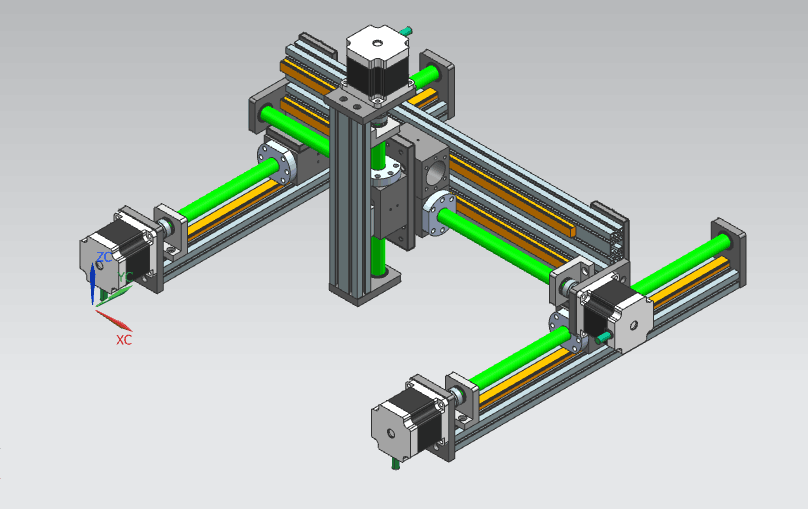
\includegraphics[width=\linewidth]{ffigures/gantry}
	\caption{Rendering of XYZ-Gantry}
	\label{fig:gant}
\end{figure}

\subsection{Stepper Motor}

A stepper motor or step motor or stepping motor is a brushless DC electric motor that divides a full rotation into a number of equal steps. The motor's position can then be commanded to move and hold at one of these steps without any position sensor for feedback (an open-loop controller), as long as the motor is carefully sized to the application in respect to torque and speed. Please refer Fig.~\ref{fig:step1}

\begin{figure}
	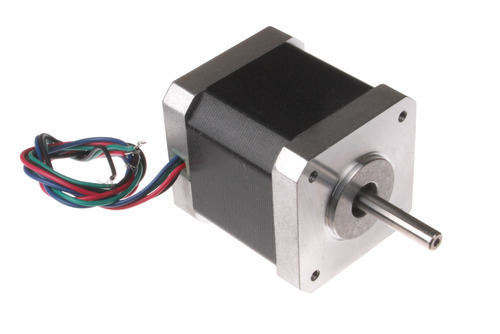
\includegraphics[scale = 4]{ffigures/stepper}
	\centering
	\caption{Stepper Motor}
	\label{fig:step1}
	
\end{figure}

\subsection{Fundamentals of Operation}

A stepper motor A bipolar hybrid stepper motor Brushed DC motors rotate continuously when DC voltage is applied to their terminals. The stepper motor is known by its property to convert a train of input pulses (typically square wave pulses) into a precisely defined increment in the shaft position. Each pulse moves the shaft through a fixed angle. Stepper motors effectively have multiple "toothed" electromagnets arranged around a central gear-shaped piece of iron. The electromagnets are energized by an external driver circuit or a micro-controller. To make the motor shaft turn, first, one electromagnet is given power, which magnetically attracts the gear's teeth. When the gear's teeth are aligned to the first electromagnet, they are slightly offset from the next electromagnet. This means that when the next electromagnet is turned on and the first is turned off, the gear rotates slightly to align with the next one. From there the process is repeated. Each of those rotations is called a "step", with an integer number of steps making a full rotation. In that way, the motor can be turned by a precise angle.

\subsection{Stepper motor driver circuits}

Stepper motor performance is strongly dependent on the driver circuit. Torque curves may be extended to greater speeds if the stator poles can be reversed more quickly, the limiting factor being a combination of the winding inductance. To overcome the inductance and switch the windings quickly, one must increase the drive voltage. This leads further to the necessity of limiting the current that these high voltages may otherwise induce. An additional limitation, often comparable to the effects of inductance, is the back-EMF of the motor. As the motor's rotor turns, a sinusoidal voltage is generated proportional to the speed (step rate). This AC voltage is subtracted from the voltage waveform available to induce a change in the current.Please refer Fig.~\ref{fig:driv}

\begin{figure}
	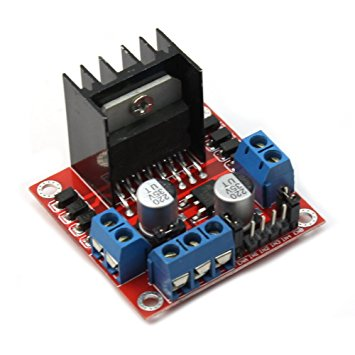
\includegraphics[scale = 0.5]{ffigures/driver}
	\centering
	\caption{Stepper Motor Driver}
	\label{fig:driv}
	
\end{figure}

\subsection{Limit Switches}

In electrical engineering a limit switch is a switch operated by the motion of a machine part or presence of an object. They are used for controlling machinery as part of a control system, as a safety interlocks, or to count objects passing a point. A limit switch is an electromechanical device that consists of an actuator mechanically linked to a set of contacts. When an object comes into contact with the actuator, the device operates the contacts to make or break an electrical connection.

Limit switches are used in a variety of applications and environments because of their ruggedness, ease of installation, and reliability of operation. They can determine the presence or absence, passing, positioning, and end of travel of an object. They were first used to define the limit of travel of an object; hence the name "Limit Switch".

A numerical control machine such as a lathe will have limit switches to identify maximum limits for machine parts or to provide a known reference point for incremental motions.

\chapter{SoC BASED CONTROL}

\section{Design of Arduino based Controller}

\subsection{ARDUINO}

\subsubsection{HARDWARE}

The Arduino Uno (refer Fig.~\ref{fig:uno}) is the most common version of Arduino family.The Arduino Uno is a micro controller board based on the ATmega328.It has 14 digital input/output pins (of which 6 can be used as PWM outputs), 6 analog inputs, a 16 MHz ceramic resonator, a USB connection, a power jack, an ICSP header, and a reset button.The Arduino Uno is great choice for beginners.It contains everything needed to support the micro controller; simply connect it to a computer with a USB cable or power it with a AC-to-DC adapter or battery to get started.The Arduino Uno is a good choice for beginners since it is easy to start with.

\begin{figure}[h!]
	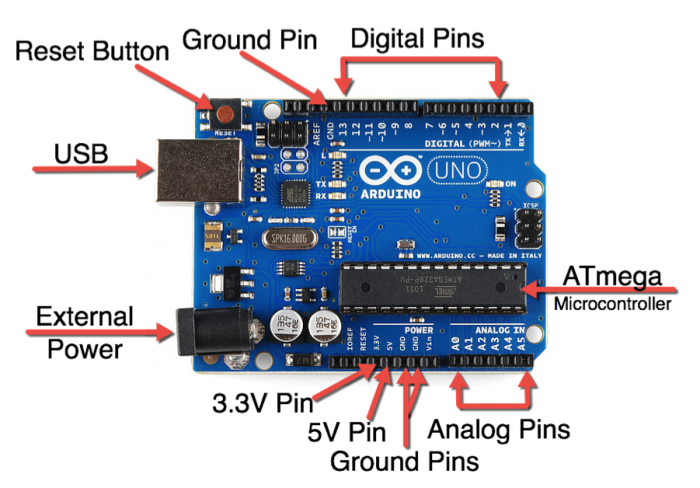
\includegraphics[scale = 0.5]{ffigures/uno}
	\centering
	\caption{Arduino UNO}
	\label{fig:uno}
	
\end{figure}

These may connect with add-on modules termed shields. Multiple and possibly stacked shields may be individually addressable via an I²C serial bus. Most boards include a 5 V linear regulator and a 16 MHz crystal oscillator or ceramic resonator. Some designs, such as the LilyPad, run at 8 MHz and dispense with the onboard voltage regulator due to specific form-factor restrictions.

\subsubsection{SOFTWARE}

Arduino IDE
A sketch is the name that Arduino uses for a program.It is the unit of code that is uploaded to and run on an Arduino board to execute the function like blinking a Led. To write a sketch,we need to install the Arduino Software known as Integrated Development Environment(IDE).

\subsection{Bluetooth Module (HC05)}

HC-05 module is an easy to use Bluetooth SPP (Serial Port Protocol) module,designed for transparent wireless serial connection setup.The HC-05 Bluetooth Module can be used in a Master or Slave configuration, making it a great solution for wireless communication.This serial port bluetooth module is fully qualified Bluetooth V2.0+EDR (Enhanced Data Rate) 3Mbps Modulation with complete 2.4GHz radio transceiver and baseband. It uses CSR Bluecore 04‐External single chip Bluetooth system with CMOS technology and with AFH (Adaptive Frequency Hopping Feature).

\begin{figure}[h!]
	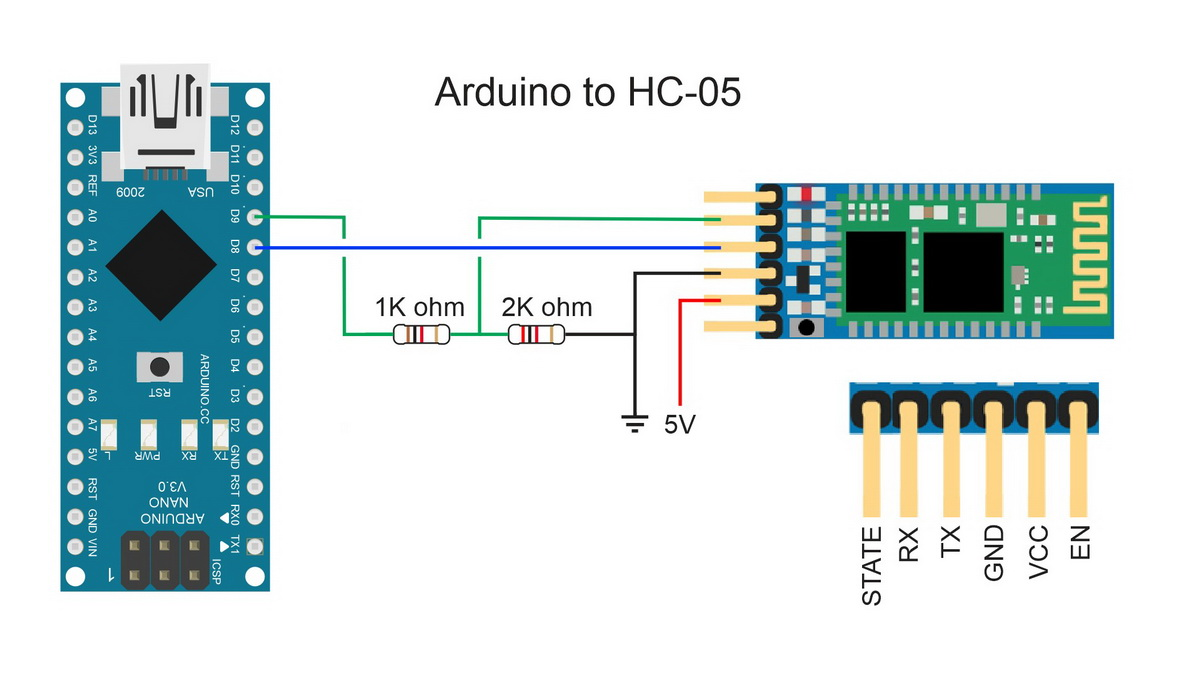
\includegraphics[scale=0.3]{ffigures/hc_conn}
	\centering
	\caption{Arduino UNO Connected to HC-05}
	\label{fig:hc05}
	
\end{figure}



\noindent The Bluetooth module HC-05 is a MASTER/SLAVE module.By default the factory setting is SLAVE.The Role of the module (Master or Slave) can be configured only by AT COMMANDS.The slave modules cannot initiate a connection to another Bluetooth device, but can accept connections.Master module can initiate a connection to other devices.The user can use it simply for a serial port replacement to establish connection between MCU and GPS, PC to your embedded project, etc.

\subsection{Joystick Module}

	\begin{figure}[h]
		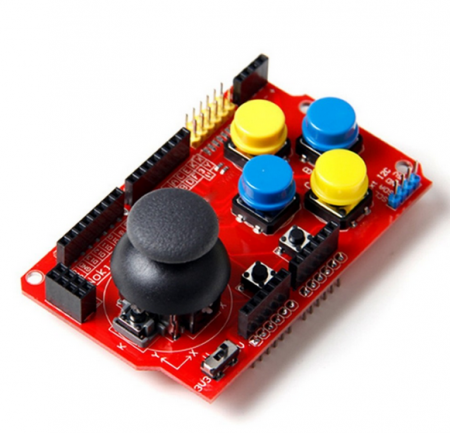
\includegraphics[scale=0.5]{ffigures/joy}
		\centering
		\caption{Joystick Shield for Arduino}
		\label{fig:joy}
	
	\end{figure}
	
A joystick is an input device consisting of a stick that pivots on a base and reports its angle or direction to the device it is controlling. A joystick, also known as the control column, is the principal control device in the cockpit of many civilian and military aircraft, either as a center stick or side-stick. It often has supplementary switches to control various aspects of the aircraft's flight. Joysticks are often used to control video games, and usually have one or more push-buttons whose state can also be read by the computer.
	
In recent times, the employment of joysticks has become commonplace in many industrial and manufacturing applications, such as; cranes, assembly lines, forestry equipment, mining trucks, and excavators. In fact, the use of such joysticks is in such high demand, that it has virtually replaced the traditional mechanical control lever in nearly all modern hydraulic control systems. Additionally, most unmanned aerial vehicles (UAVs) and submersible remotely operated vehicles (ROVs) require at least one joystick to control either the vehicle, the on-board cameras, sensors and/or manipulators.


\section{Control using Joystick Module}

The joystick module is connected to the arduino’s analog input pins as shwn in the schematic below

	\begin{figure}[h]
		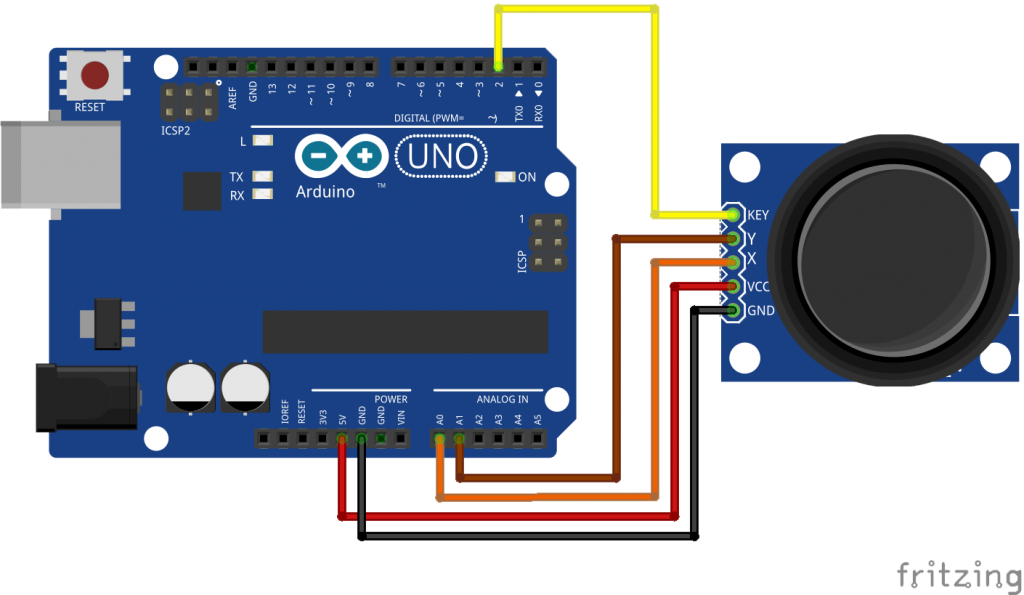
\includegraphics[width=\linewidth]{ffigures/joyschema}
		\centering
		\caption{Joystick Arduino Hookup Schematic}
		\label{fig:joysch}
	
	\end{figure}
	
The joystick module has analog out puts on X and Y axis and when pressed it can act as a switch which can be read by the Arduino.

	\begin{figure}[h]
		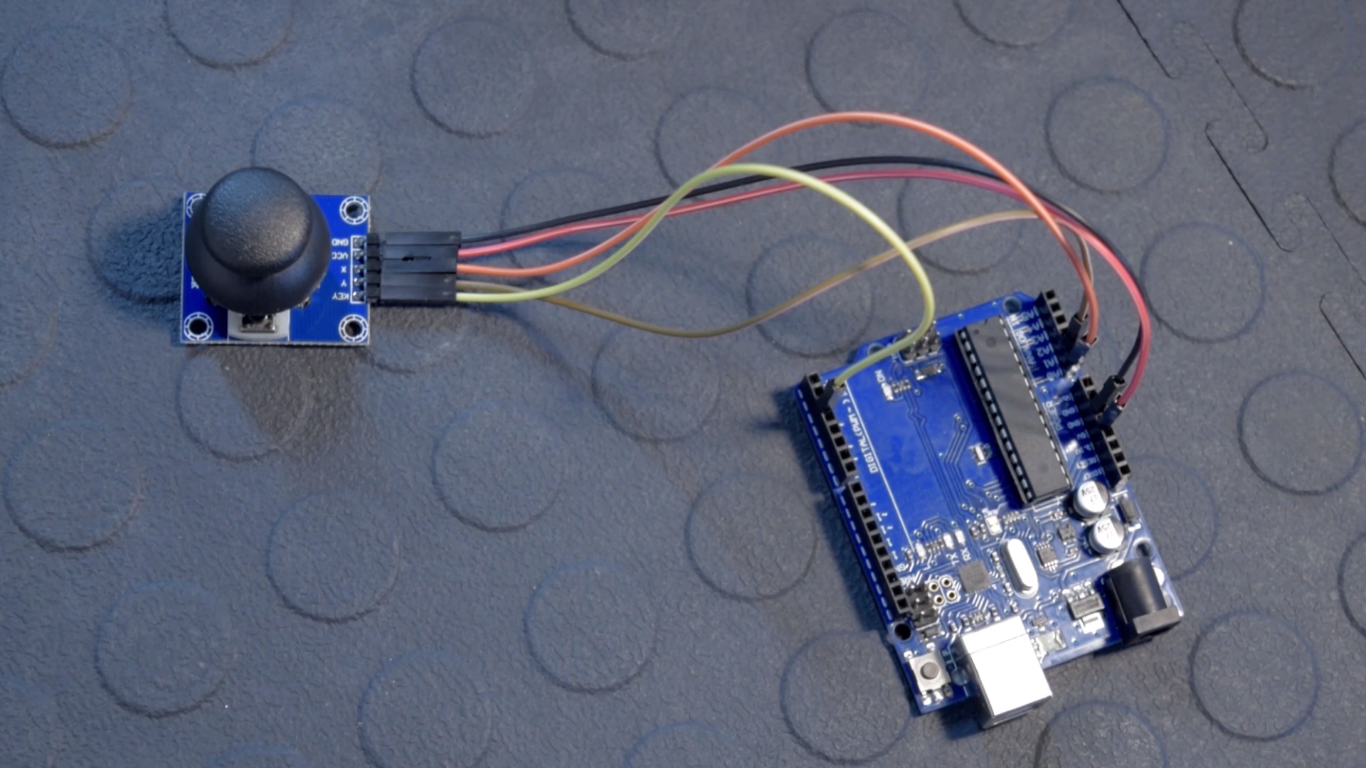
\includegraphics[width=\linewidth]{ffigures/joyschemareal}
		\centering
		\caption{Joystick connected to Arduino }
		\label{fig:joyschreal}
	
	\end{figure}
\pagebreak
The following Schematic shows how can we connect the Joystick to Arduin which in turn is connected to the Stepper Motor through an appropriate Driver

	\begin{figure}[h]
		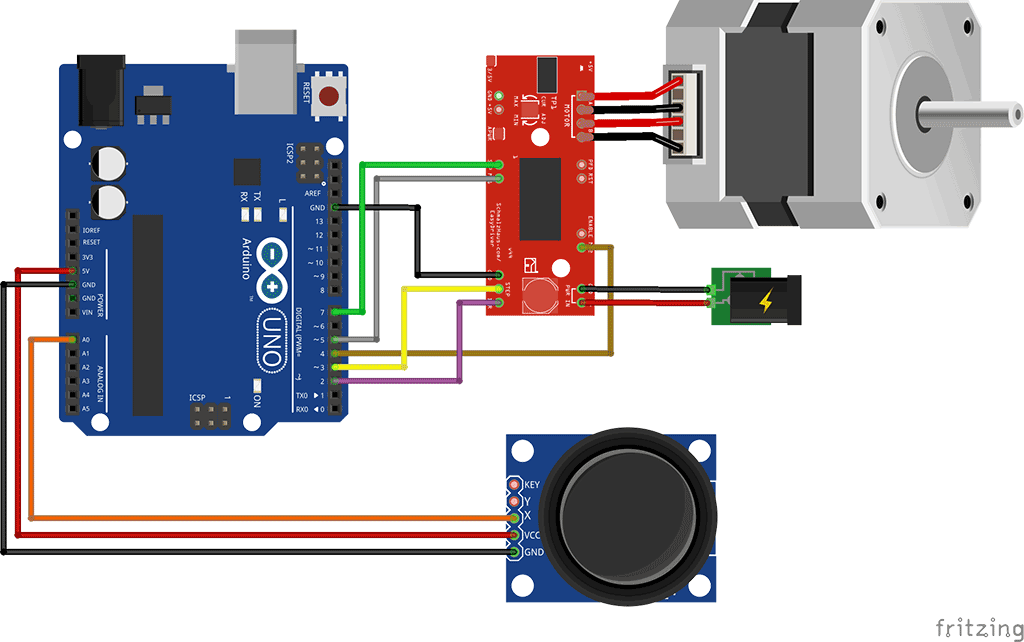
\includegraphics[width=\linewidth]{ffigures/joyardstp}
		\centering
		\caption{Joystick connected to Arduino and Stepper Motor }
		\label{fig:joyardstpp}
	
	\end{figure}
	
The following Schematic shows how we can connect the Joystick to Arduino which in turn is connected to the three Stepper Motors through the appropriate Drivers

	\begin{figure}[h]
		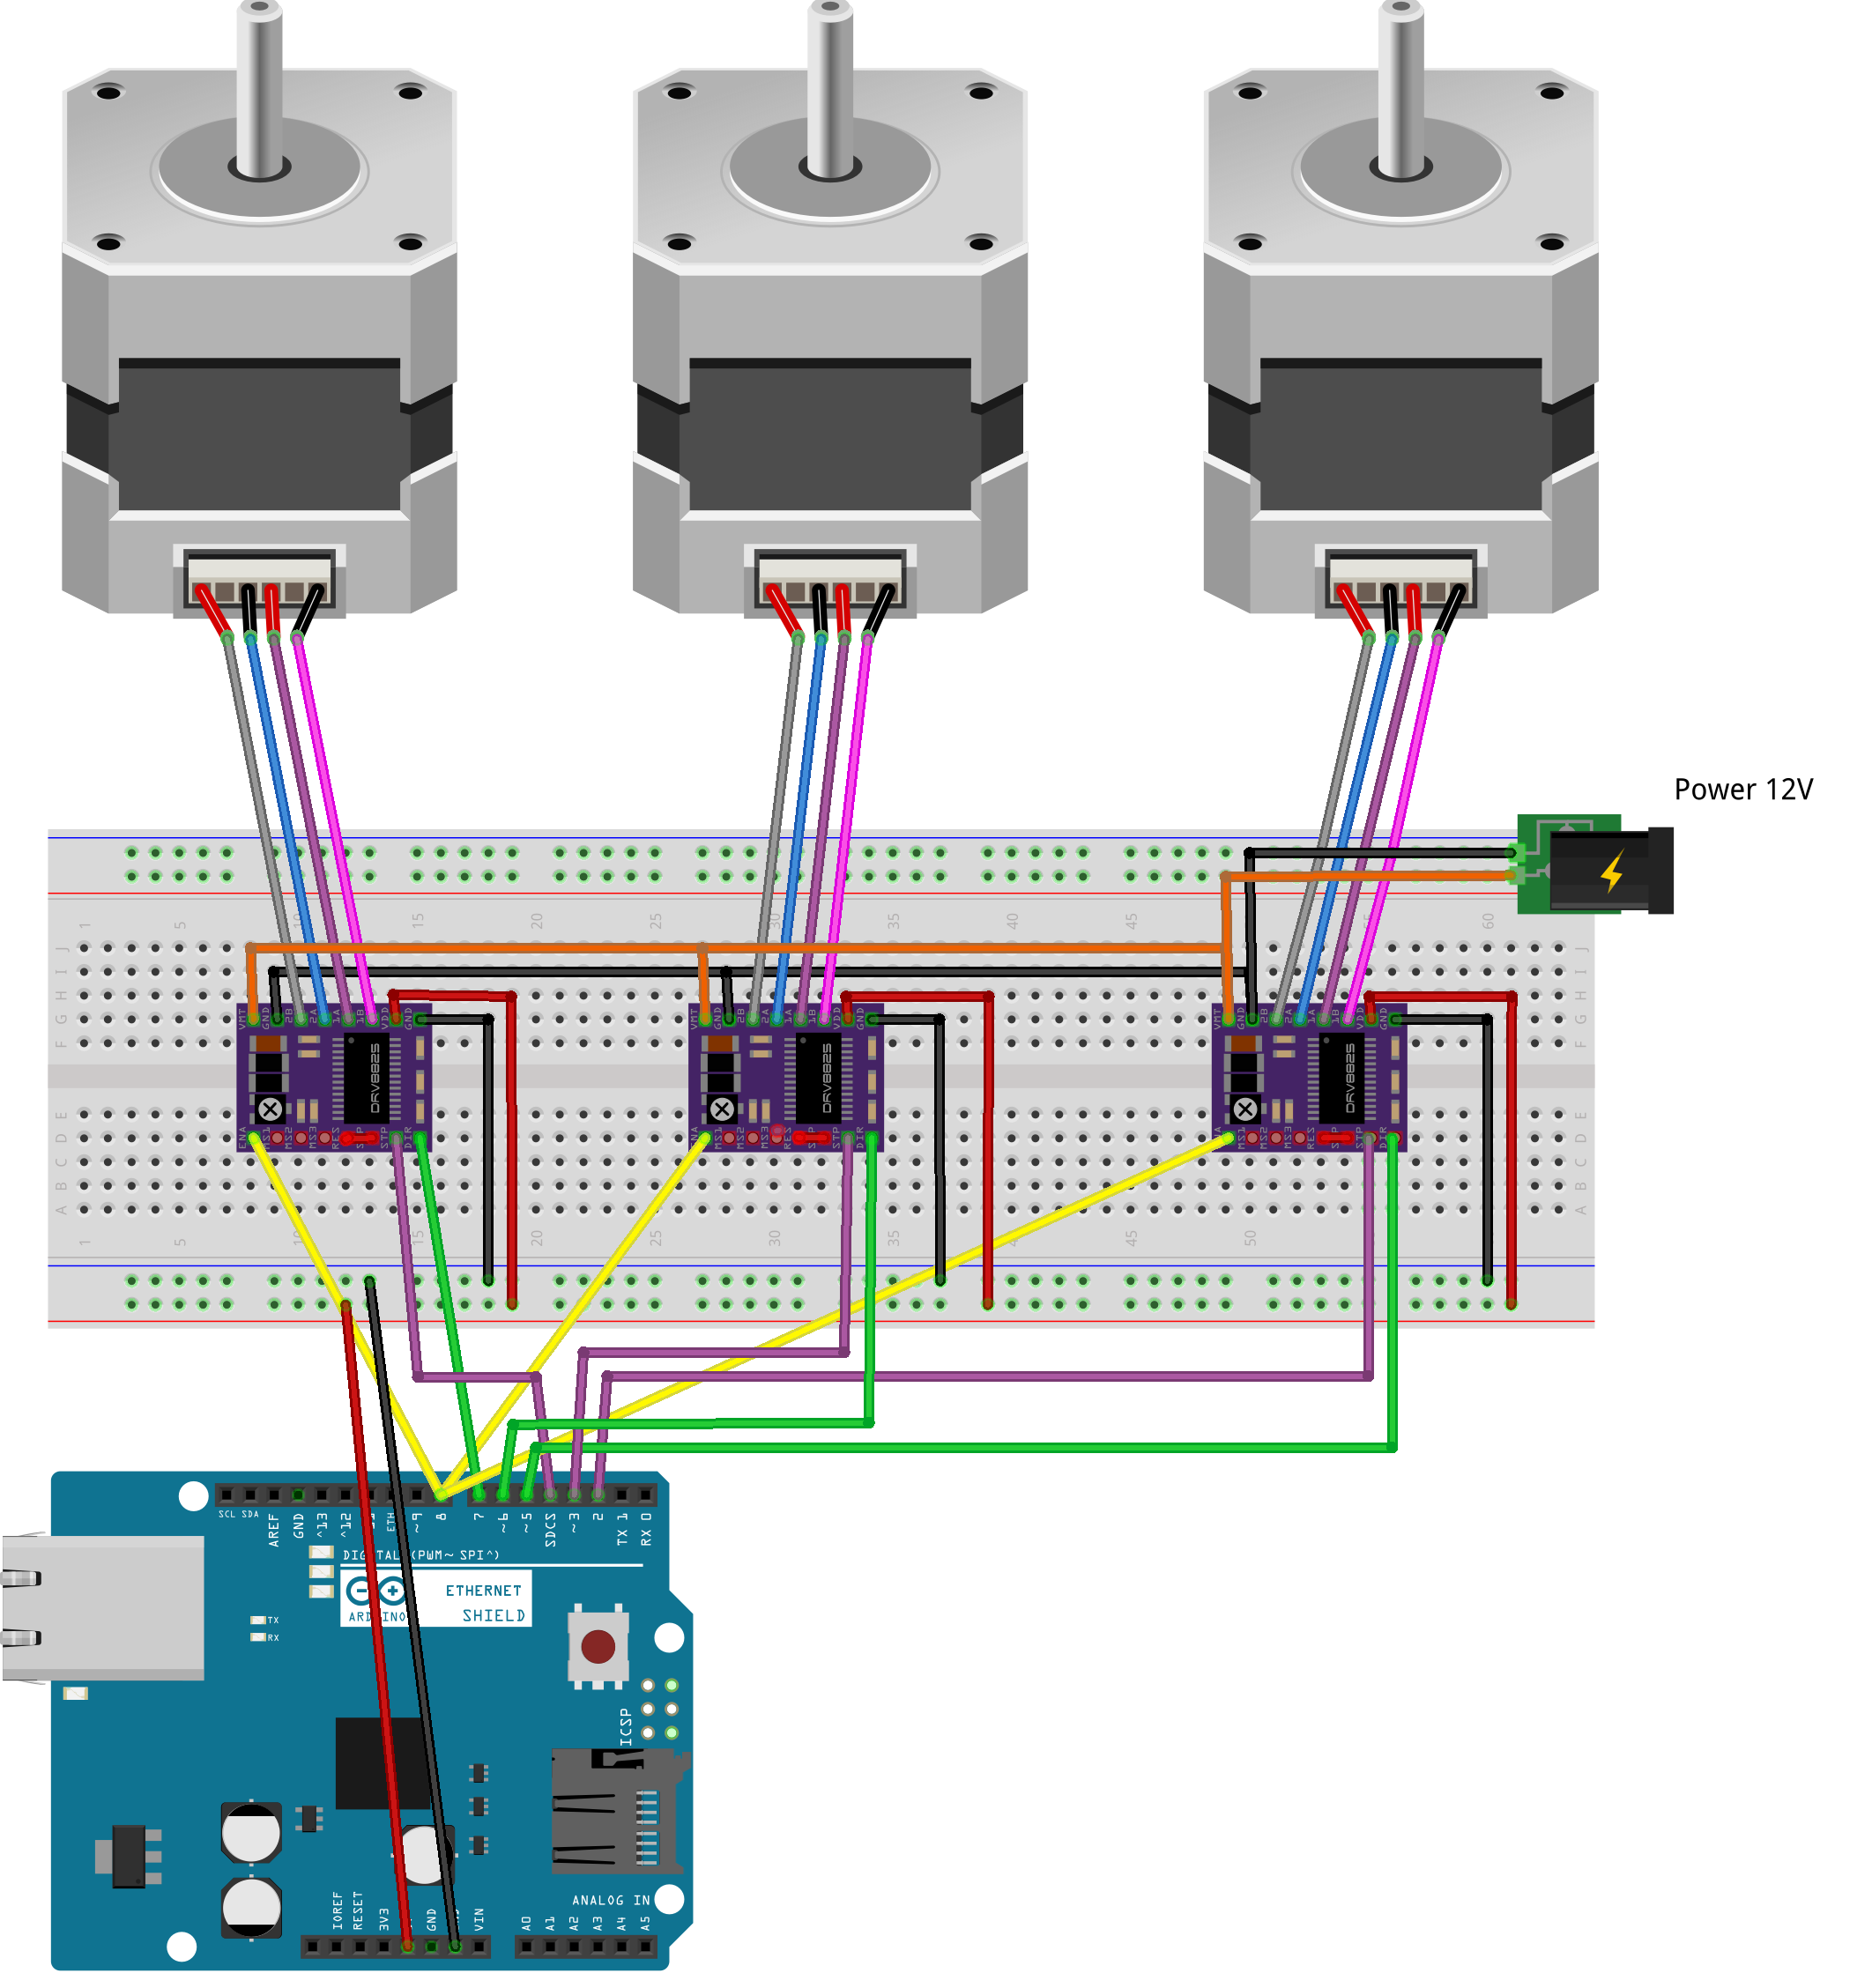
\includegraphics[width=\linewidth]{ffigures/joyardstp33}
		\centering
		\caption{Joystick connected to Arduino and 3 Stepper Motors }
		\label{fig:joyardstpp3}
	
	\end{figure}
	
	
Hence by using the module we can move in X and Y direction directly and in order to toggle X to Z direction we need to press the joystick module once and vice versa.

\emph A code snippet of the Stepper Motor

To visualize better how the motor is being controlled, we will not be using any Libraries in our code.

Instead we will be turning On and Off the Step pin of the Easy Driver and put a delay() in between to control the speed.

Since we are not using limit switches (for demnstrative experiment), the code will assume that we already positioned the belt clip in the middle position before turning on the power.

Calculations state that it takes approx. 10.25 full revolutions of the stepper motor to cover the distance between the motor and the idler pulley.  If our motor in full step mode takes 200 steps to make 1 revolution, then it will take 2050 steps to cover the distance.

So the code will assume that the belt clip is positioned in the middle at startup, or 1025 steps.

\hyperref[sec:code1]{The Code Snippet can be found by clicking on this text}


\section{Control using HC05}

HC-05 module is an easy to use Bluetooth SPP (Serial Port Protocol) module,designed for transparent wireless serial connection setup.The HC-05 Bluetooth Module can be used in a Master or Slave configuration, making it a great solution for wireless communication.

	\begin{figure}[h]
		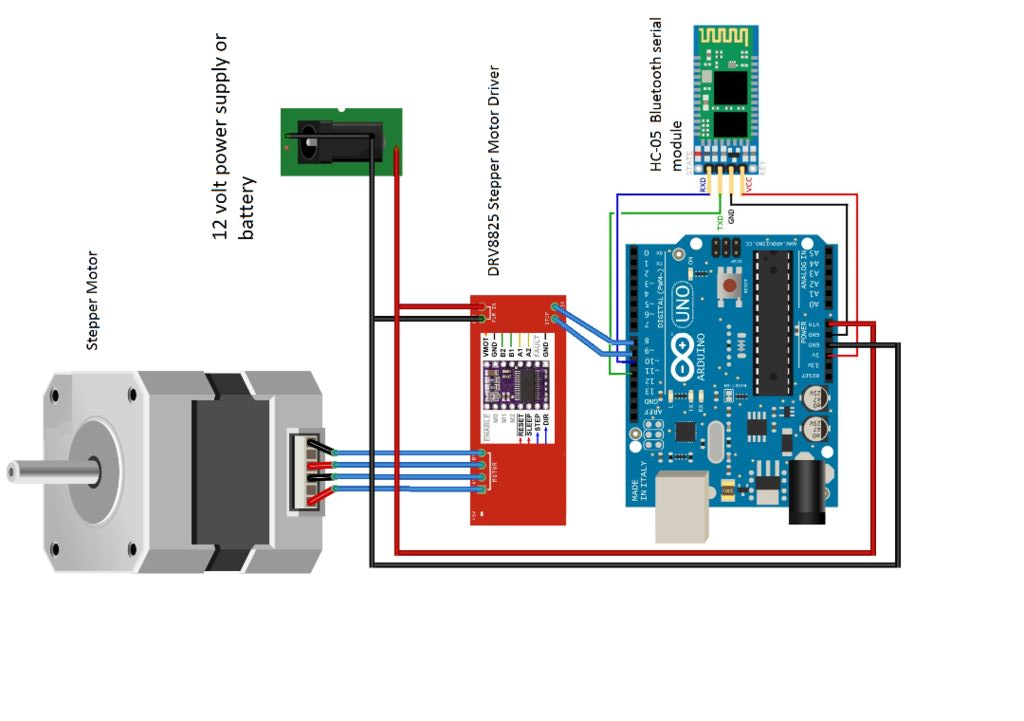
\includegraphics[width=\linewidth]{ffigures/hcardstp}
		\centering
		\caption{Schematic of Bluetooth Module HC05 and Stepper motor connected to Arduino}
		\label{fig:hcardstp}
	
	\end{figure}
	
\pagebreak

\noindent Any Bluetooth enabled smartphone can connect to the HC05 with predefined passkey. Now with the android-app available on the smartphone we can start communicating with the HC05 module. By sending commands from the smart phone we can wirelessly 

	\begin{figure}[h]
		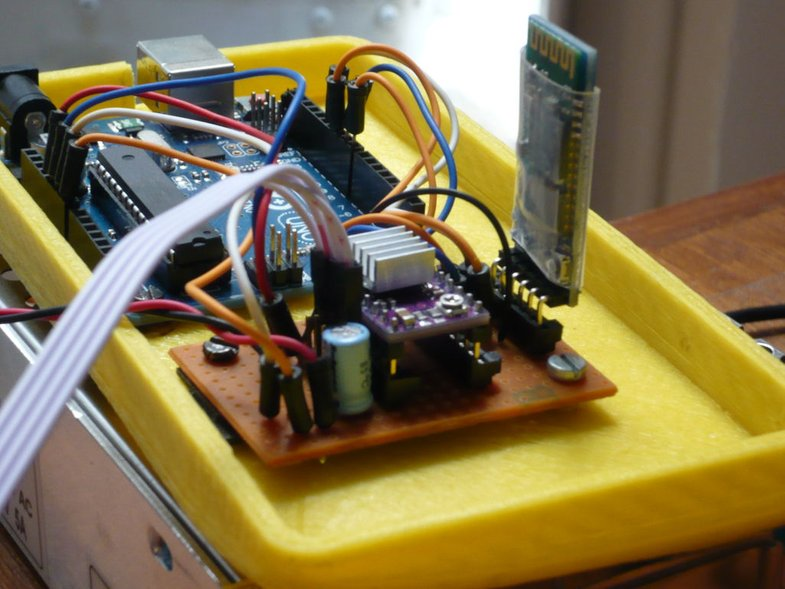
\includegraphics[width=\linewidth]{ffigures/hc05hc05}
		\centering
		\caption{Bluetooth Module HC05 and Stepper motor connected to Arduino}
		\label{fig:hc05hc05}
	
	\end{figure}
	
	
Connections between parts are shown in above picture. HC05 should be connected to pin number 10 and 11 that are configured as software serial. Also there is no connection to the reset and sleep , just jumper them and connect enable bar pin to ground of arduino. Electronics can be more compact using smaller Arduino boards like mini or nano.


\hyperref[sec:code2]{The code snippet to run a Stepper motor using Bluetooth (HC05) can be found by clicking on this text}



The Android app used to test the code

	\begin{figure}[h]
		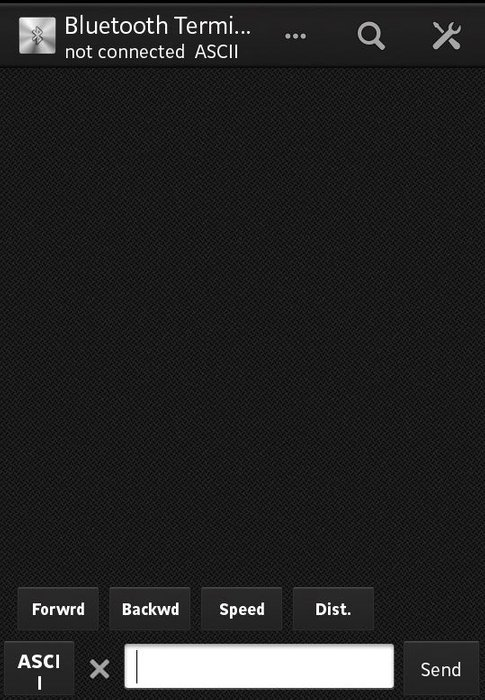
\includegraphics[scale=0.4]{ffigures/androidapp}
		\centering
		\caption{Simple Android App used to test the HC05 setup and Stepper motor}
		\label{fig:androidapp}
	
	\end{figure}
	
	
\chapter{RESULTS}

\section{Results}


Although there is a possibility of building the XYZ-Gantry system economically indigenously it will only be possible only at scale hence an economically smaller trace COTS (Commercial Off-The-Shelf) XYZ Gantry system from Chengdu Fuyu Technology Co.,Ltd was proposed

\

\noindent Arduino board was hooked with HC-05 (Bluetooth Module) and the control signals were transmitted from a mobile phone which were received by the HC-05 module which were fed to the arduino. The script running on the arduino interprets the commands received and took action as deemed appropriate according to the logic of the script. This helped in moving the XYZ positioning system be controlled in X,Y,Z axes respectively. This was preceded by hooking up a Joystick module in replacement to the Mobile (Tx) and HC05 (Rx) and tested.

\

\noindent The script running on a remote PC (Tx) was able to transmit the commands/script to the RPi (Rx) sitting at other location through internet. The API endpoint on the RPi interpreted the commands received and maneuvered the XYZ system accordingly.

\section{Conclusion}

We developed a system where by leveraging the power of SoCs we were able to control XYZ positioning system locally by turning the Arduino into a DaQ card both wired and wireless ways. We were also able to IoT-ize the system to be able to control it remotely through internet.

\section{FUTURE WORK}

By increasing the abilities of the IoT system by installing other components such as a camera to get visual feedback. A person will be able to upload a script which could run the micro-CT system and then download the end results for quick references with setting up of such features on the software side of RPi. There is a possibility of commercializing this based on the interest it generates among researchers who cannot afford to get hands on experience with such costly experimental setups.



\appendix

\chapter{APPENDIX}

\section{Stepper Motor Code}
\label{sec:code1}


\begin{lstlisting}[language=C]
#define step_pin 3  // Pin 3 connected to Steps pin on EasyDriver
#define dir_pin 2   // Pin 2 connected to Direction pin
#define MS1 5       // Pin 5 connected to MS1 pin
#define MS2 4       // Pin 4 connected to MS2 pin
#define SLEEP 7     // Pin 7 connected to SLEEP pin
#define X_pin A0    // Pin A0 connected to joystick x axis

int direction;    // Variable to set Rotation (CW-CCW) of the motor
int steps = 1025; // Assumes the belt clip is in the Middle

void setup() {
   pinMode(MS1, OUTPUT);
   pinMode(MS2, OUTPUT);
   pinMode(dir_pin, OUTPUT);
   pinMode(step_pin, OUTPUT);
   pinMode(SLEEP, OUTPUT);
   
   digitalWrite(SLEEP, HIGH);  // Wake up EasyDriver
   delay(5);  // Wait for EasyDriver wake up
   

/* Configure type of Steps on EasyDriver:
// MS1 MS2
//
// LOW LOW = Full Step //
// HIGH LOW = Half Step //
// LOW HIGH = A quarter of Step //
// HIGH HIGH = An eighth of Step //
*/

   digitalWrite(MS1, LOW);      // Configures to Full Steps
   digitalWrite(MS2, LOW);    // Configures to Full Steps
   
}

void loop() {
  while (analogRead(X_pin) >= 0 && analogRead(X_pin) <= 100) {
    if (steps > 0) {
      digitalWrite(dir_pin, HIGH);  // (HIGH = anti-clockwise / LOW = clockwise)
      digitalWrite(step_pin, HIGH);
      delay(1);
      digitalWrite(step_pin, LOW);
      delay(1);
      steps--;
    }      
  }
  
    while (analogRead(X_pin) > 100 && analogRead(X_pin) <= 400) {
      if (steps < 512) {
        digitalWrite(dir_pin, LOW);  // (HIGH = anti-clockwise / LOW = clockwise)
        digitalWrite(step_pin, HIGH);
        delay(1);
         digitalWrite(step_pin, LOW);
        delay(1);
        steps++;
      }    
      if (steps > 512) {
        digitalWrite(dir_pin, HIGH);
        digitalWrite(step_pin, HIGH);
        delay(1);
         digitalWrite(step_pin, LOW);
        delay(1);
        steps--;
      }
    }    
      
    while (analogRead(X_pin) > 401 && analogRead(X_pin) <= 600) {
      if (steps < 1025) {
        digitalWrite(dir_pin, LOW);
        digitalWrite(step_pin, HIGH);
        delay(1);
         digitalWrite(step_pin, LOW);
        delay(1);
        steps++;
      }    
      if (steps > 1025) {
        digitalWrite(dir_pin, HIGH);
        digitalWrite(step_pin, HIGH);
        delay(1);
         digitalWrite(step_pin, LOW);
        delay(1);
        steps--;
      } 
    } 

    while (analogRead(X_pin) > 601 && analogRead(X_pin) <= 900) {
      if (steps < 1535) {
        digitalWrite(dir_pin, LOW);
        digitalWrite(step_pin, HIGH);
        delay(1);
         digitalWrite(step_pin, LOW);
        delay(1);
        steps++;
      }    
      if (steps > 1535) {
        digitalWrite(dir_pin, HIGH);
        digitalWrite(step_pin, HIGH);
        delay(1);
         digitalWrite(step_pin, LOW);
        delay(1);
        steps--;
      }    
    }   
   
    while (analogRead(X_pin) > 900 && analogRead(X_pin) <= 1024) {
      if (steps < 2050) {
        digitalWrite(dir_pin, LOW);
        digitalWrite(step_pin, HIGH);
        delay(1);
         digitalWrite(step_pin, LOW);
        delay(1);
        steps++;
      }
    }
}
\end{lstlisting}


\section{HC05 and Stepper Motor}
\label{sec:code2}
\begin{lstlisting}
// This program shows how to control arduino from Bluetooth for controlling Stepper Motor

// arduino>>bluetooth
// D10   >>>  Rx
// D11   >>>  Tx
//Written By Hesam 
//for Bluetooth connection: http://www.genotronex.com/

// you will need arduino 1.0.1 or higher to run this sketch

#include <SoftwareSerial.h>// import the serial library

SoftwareSerial Genotronex(10, 11); // RX, TX



int dirPin = 8;
int stepperPin = 9;
String inData="";
String dinData="";
int sliderspeed=1;
int sliderdist=1;
int BluetoothData; // the data from Android phone

void setup() {

  Genotronex.begin(9600);
  Genotronex.println("Bluetooth On . Slider ready..");

   pinMode(dirPin, OUTPUT);
 pinMode(stepperPin, OUTPUT);
  
}
 void step(boolean dir,int steps,int sldrspeed){
   // define a function to move slider based on speed, direction and distance
 digitalWrite(dirPin,dir);
 delay(5);
 for(int i=0;i<(steps);i++){
    for(int j=0;j<32;j++){
   digitalWrite(stepperPin, HIGH);
   delayMicroseconds(200+(sldrspeed-1)*2000); // for adjustment of speed we just put proper delay
   digitalWrite(stepperPin, LOW);
   delayMicroseconds(200+(sldrspeed-1)*2000);
    }
 }
}
void loop() {
  
  // put your main code here, to run repeatedly:
   if (Genotronex.available()){
BluetoothData=Genotronex.read();   // recieve the commands from Android phone
   if(BluetoothData=='F'){   
    Genotronex.println("Move forward ! ");
  
    step(true,200*sliderdist,sliderspeed);
   
 delay(500);
   Genotronex.println("Stoped ! ");
  
   }
  if (BluetoothData=='B'){
   Genotronex.println("Move backward ! ");
  step(false,200*sliderdist,sliderspeed);
 delay(500);
  Genotronex.println("Stoped ! ");
  }
    
      if (BluetoothData=='S'){
  
    
      Genotronex.println("Enter speed ! ");
      
      while(!Genotronex.available()){
      delay(3);
      }
 
  
        char recieved = Genotronex.read();
      sliderspeed= recieved-48; 
 
    
 
            Genotronex.print("Speed is: ");
            Genotronex.print(sliderspeed);
 
    
      
      } 
          if (BluetoothData=='D'){
  
    
      Genotronex.println("Enter distance ! ");
      
           while(!Genotronex.available()){
      delay(3);
      }
     
        char recieved = Genotronex.read();
        sliderdist= recieved-48; 

    
            Genotronex.print("Distance is: ");
            Genotronex.print(sliderdist);

      } 
      
}
delay(100);// prepare for next data ...
}
\end{lstlisting}


Just put in text as you would into any chapter with sections and
whatnot.  Thats the end of it.

%%%%%%%%%%%%%%%%%%%%%%%%%%%%%%%%%%%%%%%%%%%%%%%%%%%%%%%%%%%%
% Bibliography.

\begin{singlespace}
  \bibliography{refs}
\end{singlespace}


%%%%%%%%%%%%%%%%%%%%%%%%%%%%%%%%%%%%%%%%%%%%%%%%%%%%%%%%%%%%
% List of papers

\listofpapers

\begin{enumerate}  
\item Authors....  \newblock
 Title...
  \newblock {\em Journal}, Volume,
  Page, (year).
\end{enumerate}  

\end{document}
